%
% main.tex -- Paper zum Thema <antennen>
%
% (c) 2020 Autor, OST Ostschweizer Fachhochschule
%
% !TEX root = ../../buch.tex
% !TEX encoding = UTF-8
%
\chapter{Antennen\label{chapter:antennen}}
\kopflinks{Antennen}
\begin{refsection}
\chapterauthor{Baris Catan und Jannis Gull}

Das Ziel dieses Kapitels ist, den Wirkungsgrad einer dreieckigen Loop-Antenne mittels 
Formoptimierung zu erhöhen. Für die Umsetzung dieser Problemstellung wird 
eine direkte Methode der Variation, in diesem Fall das Verfahren nach Ritz, 
verwendet.

%
% antennenAllgemein.tex 
%
% 
%
% !TEX root = ../../buch.tex
% !TEX encoding = UTF-8
%

\section{Antennen\label{antennen:antennenAllgemein}}
\kopfrechts{Antennen}
Antennen sind in der heutigen technologischen Welt unverzichtbar.
Sie sind in zahlreichen Formen und Varianten in fast allen
elektronischen Geräten zu finden. Ihre primäre Funktion besteht
darin, elektromagnetische Wellen von einer leitungsgebundenen Form
\index{elektromagnetische Wellen}%
\index{Wellen, elektromagnetische}%
in freie Wellen im Raum zu verwandeln. Dieser Vorgang ist essenziell
für die Kommunikation, da er die Übertragung von Signalen über große
Distanzen ermöglicht. Ein weiterer entscheidender Aspekt von Antennen
ist ihre Reziprozität: Sie können sowohl Signale senden als auch
\index{Reziprozität}%
empfangen. Dabei wandeln sie freie Wellen aus dem Raum zurück in
leitungsgebundene Wellen. Diese Fähigkeit macht Antennen zu einem
grundlegenden Element der modernen Kommunikationstechnologie. Ohne
sie wäre die drahtlose Übertragung von Daten und Signalen, wie wir
sie heute kennen, undenkbar.

Eine genauere Erklärung von elektromagnetischen Wechselwirkungen findet der Leser im Kapitel \ref{chapter:maxwell},
welches sich mit den Maxwell-Gleichungen befasst. 
\index{Maxwell-Gleichungen}%

\subsection{Loop-Antennen\label{antennen:antennenAllgemein_loop}}


Eine Loop-Antenne hat eine recht simple Funktionsweise. Sie besteht aus einem Stück Draht wie in Abbildung \ref{antennen:loopAntenne} dargestellt. Die Loop-Antenne kann, nicht wie der Name impliziert, verschiedenste Formen annehmen. Durch den Leiter wird ein Signal geführt, das in der aufgespannten Fläche ein magnetisches Feld induziert. Dieses Feld wird durch Anpassung der Signalamplitude verändert. Eine solche Änderung kann als Information angesehen werden, die sich nun im freien Raum fortbewegt.

\begin{figure}
	\centering
	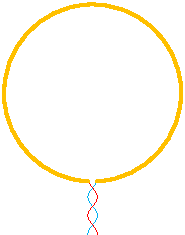
\includegraphics{papers/antennen/images/loopAntenne.pdf}
	\caption{Form einer typischen Loop-Antenne}
	\label{antennen:loopAntenne}
\end{figure}

\subsection{Eigenschaften\label{antennen:antennenEigenschaften}}
Der Wirkungsgrad
\index{Wirkungsgrad}%
\begin{equation}
	\eta=\frac{P\textsubscript{rad}}{P\textsubscript{tot}},
	\label{antennen:Wirkungsgrad}
\end{equation}
auch Effizienz genannt, kann mittels der eingespeisten Gesamtleistung
der Antenne $P\textsubscript{tot}$ und der abgestrahlten Leistung
$P\textsubscript{rad}$ berechnet werden. Eine Leistung $P$ entspricht
dem elektrischen Widerstand multipliziert mit der Stromstärke im
Quadrat. Nach Vereinfachung ergibt sich, dass die Effizienz
\begin{equation}
	\eta=\frac{P\textsubscript{rad}}{P\textsubscript{tot}}=\frac{R\textsubscript{rad}\cdot{I^2}}{R\textsubscript{tot}\cdot{I^2}}=\frac{R\textsubscript{rad}\cdot{I^2}}{(R\textsubscript{rad}+R\textsubscript{loss})\cdot{I^2}}=\frac{R\textsubscript{rad}}{R\textsubscript{rad}+R\textsubscript{loss}}
	\label{antennen:Wirkungsgradkomplett}
\end{equation}
nur noch vom Verlustwiderstand und dem Strahlungswiderstand abhängig ist. $R\textsubscript{rad}$ und $R\textsubscript{loss}$ werden wie folgt definiert:
\index{Verlustwiderstand}%
\index{Strahlungswiderstand}%
\begin{align}
	R_{\text{rad}} &= 31171 \Omega \cdot \bigg( \frac{A}{\lambda^2} \bigg)^2 \tag{20.3} \label{antennen:Rrad} \\
	R_{\text{loss}} &= \frac{\rho \cdot l}{r^2 \cdot \pi}. \tag{20.4} \label{antennen:Rloss}
\end{align}

Die Formel \eqref{antennen:Rrad} für die Berechnung des
Strahlungswiderstands wurde aus Fachliteratur \cite{antennen:antennaTheory}
übernommen, welche erklärt, dass die ``magische'' Konstante in
\eqref{antennen:Rrad} durch elektrodynamische Gesetzte entsteht.
Sie gilt für die verschiedensten Formen von Loop-Antennen, welche
einen kleinen Umfang  $l$ < $\lambda$/10 aufweisen. $A$ wird hierbei
als aufgespannte Fläche definiert, während $\lambda$ der Wellenlänge
entspricht. Eine Wellenlänge
\setcounter{equation}{4}
\begin{equation}
	\lambda = \frac{c}{f}
	\label{antennen:lambda}
\end{equation}
entspricht dem Verhältnis der materialspezifischen Lichtgeschwindigkeit $c$ und der Einsatzfrequenz $f$.
\index{Lichtgeschwindigkeit}%
\index{c@$c$}%
Der Verlustwiderstand wird aus dem spezifischen Widerstand $\rho$, dem Umfang $l$ und dem Leiterradius $r$ berechnet. Die Formeln \eqref{antennen:Rrad} und \eqref{antennen:Rloss} können in dieser Arbeit vereinfacht werden, da die Einsatzfrequenz und die Drahteigenschaften als konstant und gegeben angesehen werden können. Es resultieren die Ausdrücke 
\begin{align}
	R_{\text{rad}} &= k_{\text{1}} \cdot A^2 \tag{20.6} \label{antennen:Rrad_konst} \\
	R_{\text{loss}} &= k_{\text{2}} \cdot l \tag{20.7} \label{antennen:Rloss_konst}
\end{align}
für die beiden Widerstände. $k\textsubscript{1}$ und $k\textsubscript{2}$ werden als Konstanten betrachtet. Eingesetzt in \eqref{antennen:Wirkungsgradkomplett} ergibt sich
\setcounter{equation}{7}
\begin{equation}
\eta
=
\frac{
k\textsubscript{1}\cdot{A^2}
}{
k\textsubscript{1}\cdot{A^2}+{k\textsubscript{2}\cdot{l}}
}
=
\frac{1}{
1+\displaystyle\frac{k\textsubscript{2}\cdot{l}}{k\textsubscript{1}\cdot{A^2}}
}
	\label{antennen:Wirkungsgradeingesetzt}
\end{equation}
für den Wirkungsgrad.

%
% problemstellung.tex 
%
% 
%
% !TEX root = ../../buch.tex
% !TEX encoding = UTF-8
%

\section{Problem\label{antennen:problemstellung}}
\rhead{Problem}

bla bla antennen

knknknkn

kjkjkj
%
% unserRitz.tex 
%
% 
%
% !TEX root = ../../buch.tex
% !TEX encoding = UTF-8
%

\section{Das Ritz-Verfahren\label{antennen:ritzGrundsätzlich}}

Wie schon sehr oft in diesem Buch erwähnt, gibt es das Problem, dass man für ein Funktional
\begin{equation}
I(y)
=
\int_{x_1}^{x_2}L(x,y(x),y'(x))\,dx
\label{antennen:normalesFunktional}
\end{equation}
eine Funktion $y(x)$ finden muss, welche das Funktional extremal macht.
Solch eine Funktion ist die Lösung der Euler-Lagrange Differentialgleichung
\begin{equation}
\frac{\partial L}{\partial y} - \frac{d}{dx} \left( \frac{\partial L}{\partial y'} \right) = 0.
\label{antennen:el-DGL}
\end{equation}
Wenn diese Gleichung \eqref{antennen:el-DGL} 
jedoch analytisch nicht lösbar ist, kommt das Verfahren nach Ritz ins Spiel.

\subsection{Approximationsfunktion nach Ritz\label{antennen:approxFunkt}}

Aus der Fourier-Theorie weiss man, dass
periodische Funktionen $f(t)$ als Linearkombination von anderen Funktionen, 
im Sinne der Fourierreihe als
%todo WHY SIND KLAMMERN GROSS? CHECKS NID
\begin{equation}
f(t)
=
\frac{a_0}{2}+\sum_{n=1}^{\infty}[a_n\cos(n \omega_f t )+b_n\sin(n \omega_f t)]
\label{antennen:fourier}
\end{equation}
beschrieben werden können.

Eine ähnliche Idee wird beim Verfahren nach Ritz angewendet.
Es wird eine Approximationsfunktion in der Form
\begin{equation}
y(x)=\sum_{k=1}^n a_k \psi_k(x)
\label{antennen:ritzFunkt}
\end{equation}
definiert. Die Funktionen $\psi_k(x)$ und Koeffizienten $a_k$, oder
wie in der Welt des Verfahrens nach Ritz,  
\em Koordinatenfunktionen $\psi_k(x)$ \em und \em Koordinaten \em $a_k$.
Im weiteren Verlauf jedoch behalten wir die intuitiveren, zuerst genannten Namen.

\subsection{Mögliche Approximationsfunktionen\label{antennen:approxBsp}}

Je nach Problemstellung gibt es bessere oder schlechtere Approximationsfunktionen.
Mögliche ausgeschriebene Funktionen können so aussehen:
\begin{equation}
	\begin{aligned}
		\text{Potenz-Entwicklung: }
		y(x)
		&=
		a_0+a_1 x+a_2 x^2+\cdots+a_n x^n \\
		\text{Fourier-Entwicklung: } 
		y(x)
		&=
		a_0+a_1\cos(x)+b_1\sin(x)+\cdots+a_n\cos(n x)+b_n\sin(n x)\\
		\text{Exponential-Entwicklung: } 
		y(x)
		&=
		a_1 e^{\lambda x}+a_2 e^{-\lambda x}+\cdots+a_n e^{(-1)^n \lambda}
	\end{aligned}
\label{antennen:approxFunktBsp}
\end{equation}

Das Ziel ist es schlussendlich, das Problem so genau wie nötig mit so wenig
Koeffizienten wie möglich auszudrücken.


%
% ritzAufProblem.tex 
%
% 
%
% !TEX root = ../../buch.tex
% !TEX encoding = UTF-8
%



\section{Ritz-Verfahren für das Antennenproblem\label{antennen:ritzAnw}}

%todo CHAPTER REFERENZ
Wie in \ref{antennen:Geom} erwähnt, kann dank der Symmetrie das Problem nur auf eine Ecke abbildet werden. 
Diese Ecke setze man nun geschickt wie in der Abbildung \ref{antennen:koordSysBsp} zu sehen 
in ein Koordinatensystem, welches erlaubt das Problem genauer zu analysieren.
%TODO bild ist weit weg  ILLEGAL
\begin{figure}
	\centering
	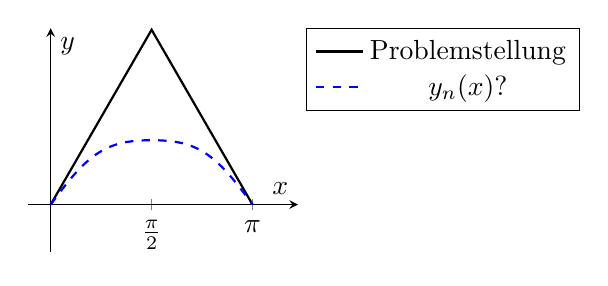
\begin{tikzpicture}
		\begin{axis}[
			scale=0.5,
			axis lines=middle,
			xlabel={$x$},
			ylabel={$y$},
			xtick={0, 1.5708, 3.14159},
			xticklabels={0, $\frac{\pi}{2}$, $\pi$},
			ytick=\empty,
			enlargelimits,
			clip=false,
			xmin=0, xmax=3.5,
			ymin=0, ymax=2,
			domain=0:pi, 
			samples=100,
			legend pos=outer north east,
			axis equal
			]
			% 3eck spitze
			\addplot[thick] coordinates {(0,0) (1.5708, pi*1.732/2) (3.14159, 0)};
			\addlegendentry{Problemstellung}
			
			\addplot[thick, blue, dashed, domain=0:3.14159, samples=100] {1.0882345*sin(deg(x))+0.0866761*sin(3*deg(x))};
			\addlegendentry{$y_n(x)?$}
		\end{axis}
	\end{tikzpicture}
	\caption{Problemstellung im Koordinatensystem}
	\label{antennen:koordSysBsp}
\end{figure}

Um die Effizienz $\eta$ zu optimieren, soll man mit der Approximationsfunktion
$y_n(x)$, wie im Kapitel \ref{antennen:Geom} erwähnt, die Fläche $A$ 
maximieren und die Länge $l$ minimieren.

\subsection{Ideale Approximationsfunktion\label{antennen:unsereApproxFunkt}}

Bei diesem Problem ist zu erwarten, dass die Lösung eine glatte und symmetrische
Funktion sein wird, somit ergibt sich
\begin{equation}
	y_n(x)
	= 
	\sum_{k=1}^n a_k\sin((2k-1)x)
	\label{antennen:unserRitz}
\end{equation}
als ideale Approximationsfunktion. 

Diese Entwicklung wird auch Sinus-Fourier Reihe genannt
und wenn man diese für $n=2$ ausschreibt, ergibt sich
\begin{equation}
	y_n(x)
	=
	a_1\sin(x)+a_2\sin(3x)
	\label{antennen:approxFunktn2}
\end{equation}
als Approximationsfunktion. Im weiteren Verlauf ist $y_n(x)$ \eqref{antennen:approxFunktn2} 
unsere endgültige Approximationsfunktion, mit der wir die Problemstellung angehen werden.

\subsection{Nebenbedingungen von $y_n(x)$\label{antennen:nebenbedRitz}}

Eine Nebenbedingung ist es, dass bei $y_n(0)$ und $y_n(\pi)$ die Funktion null sein muss.
Diese Nebenbedingung ist sehr wichtig für die Stetigkeit der finalen Antennenform, die wir optimieren.

Die Sinus-Fourier Reihe \eqref{antennen:unserRitz} hat eine weitere gute Eigenschaft, 
die ersichtlich wird, wenn man das gleiche Koordinatensystem wie bei der Abbildung \ref{antennen:koordSysBsp}
benützt und $y_n(x)$ mit beispielsweise den Koeffizienten $a_1=a_2=1$ plottet.

%TODO bild ist weit weg  ILLEGAL
\begin{figure}
	\centering
	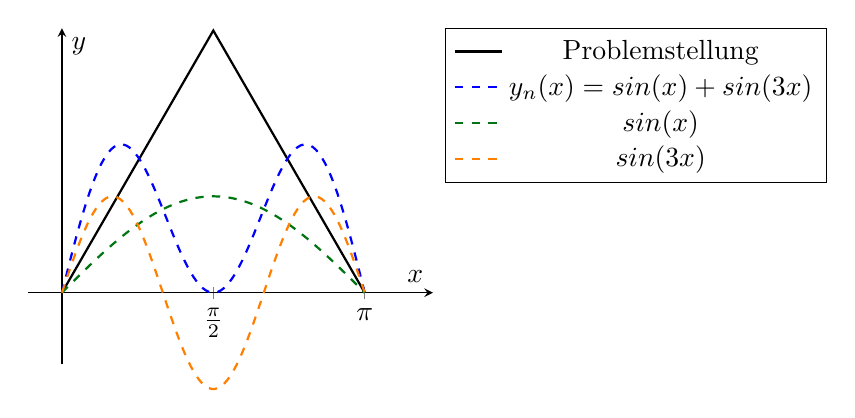
\begin{tikzpicture}
		\definecolor{clrGreen}{RGB}{0, 117, 18}
		\begin{axis}[
			scale=0.75,
			axis lines=middle,
			xlabel={$x$},
			ylabel={$y$},
			xtick={0, 1.5708, 3.14159},
			xticklabels={0, $\frac{\pi}{2}$, $\pi$},
			ytick=\empty,
			enlargelimits,
			clip=false,
			xmin=0, xmax=3.5,
			ymin=0, ymax=2,
			domain=0:pi, 
			samples=100,
			legend pos=outer north east,
			axis equal
			]
			% 3eck spitze
			\addplot[thick] coordinates {(0,0) (1.5708, pi*1.732/2) (3.14159, 0)};
			\addlegendentry{Problemstellung}
			
			\addplot[thick, blue, dashed, domain=0:3.14159, samples=100] {sin(deg(x))+sin(3*deg(x))};
			\addlegendentry{$y_n(x) = sin(x)+sin(3x)$}
			
			\addplot[thick, clrGreen, dashed, domain=0:3.14159, samples=100] {sin(deg(x))};
			\addlegendentry{$sin(x)$}
			
			\addplot[thick, orange, dashed, domain=0:3.14159, samples=100] {sin(3*deg(x))};
			\addlegendentry{$sin(3x)$}
		\end{axis}
	\end{tikzpicture}
	\caption{Nebenbedingungen im Koordinatensystem}
	\label{antennen:nebenbedGrafik}
\end{figure}

In der Abbildung \ref{antennen:nebenbedGrafik} ist zu sehen, dass dank der Punktsymmetrie 
der ungeraden Sinus-Funktionen, die Nebenbedingungen
\begin{equation}
	\begin{aligned}
		y_n(0)
		&=
		0
		\\
		y_n(\pi)
		&=
		0
	\end{aligned}
\label{antennen:nebenbed3eck}
\end{equation}
\em immer erfüllt \em sind. Im weiteren Verlauf werden diese 
Nebenbedingungen somit nicht mehr beachtet.

\subsection{Die Lagrange-Funktion \label{antennen:lagrangeFunktionen}}

%Die beste Fläche ist auch gerade die beste Fläche im quadrat \qed

Abstrahieren wir das Problem nun ein bisschen. Anstelle der Fläche $A$ reden wir nun von 
der Funktion $f$ und aus der Länge $l$ wird die Nebenbedingung $n$. 

An dieser Stelle sind unsere Koeffizienten $a_k$ konkret zu bestimmen. 
Somit sind die neu erwähnten Funktionen 

\begin{equation}
\begin{aligned}
	A
	\rightarrow
	f(a_1,\ldots,a_k)
	\rightarrow
	f(a_1,a_2)
	&=
	\int\limits_{0}^{\pi} y_n(x,a_1,a_2)\, dx
	\\
	l
	\rightarrow
	n(a_1,\ldots,a_k)
	\rightarrow
	n(a_1,a_2)
	&=
	\int\limits_{0}^{\pi} \sqrt{1+y_n'(x, a_1, a_2)^2}\, dx
\end{aligned}
\label{antennen:lagrangeNamen}
\end{equation}
auch in deren Abhängigkeit in \eqref{antennen:lagrangeNamen} zu sehen. Wie schon erwähnt, 
ist das Problem hier auf zwei Koeffizienten beschränkt. 

Die Fläche unter der Kurve ergibt sich aus dem Integral der Funktion, 
währenddessen man für die Länge, also den oberen Rand der Funktion, die 
erste Ableitung auch noch zusätzlich braucht.

Die Nebenbedingung $n$ setzen wir nun gleich einer konstanten Länge $l$
\begin{equation}
n(a_1, a_2)
=
l
\label{antennen:constNebenbed}
\end{equation}
und wie jede gute Nebenbedingung setzen wir diese noch gleich null :

\begin{equation}
\begin{aligned}
	n(a_1, a_2) - l
	&=
	0
	\\
	n(a_1, a_2, l)
	&=
	0.
\label{antennen:fertigeNebenbed}
\end{aligned}
\end{equation}
Nun kann man die endlichdimensionale Lagrange-Funktion

\begin{equation}
F(x,a_1,a_2,\lambda)
= 
f(a_1,a_2)+\lambda \: n(a_1,a_2, l)
\end{equation}
definieren. Dazu wird die Funktion $f$ mit der Lagrange-Nebenbedingung $\lambda \: n (a_1,a_2, l)$ addiert.

\subsection{Lagrange-Gleichungssystem\label{antennen:lagrangeGLsys}}

Nun möchte man die endlichdimensionale Lagrange-Funktion $F$ ableiten und gleich 0 setzen. Das heisst in diesem Kontext
den Gradienten

\begin{equation}
	\nabla F = \vec{0} \,
	\left\{ \:
	\begin{aligned}
		\frac{\partial L}{\partial a_1} = 0 \\
		\frac{\partial L}{\partial a_2} = 0
	\end{aligned}
	\right.
	\label{antennen:lagrangeGrad}
\end{equation}
berechnen und dem Nullvektor gleichsetzen. Dabei entsteht hier ein 
$n+1$ dimensionales Gleichungssystem aus \eqref{antennen:lagrangeGrad} und \eqref{antennen:fertigeNebenbed}. 
Wobei $n$ die Anzahl der Koeffizienten ist.

An dieser Stelle wird ersichtlich, was diese Kapitel von den anderen unterschiedet. Dank dem Verfahren nach Ritz konnten wir ein unendlich dimensionales
Problem wie z. B. im Kapitel \ref{buch:chapter:nebenbedingungen}, in ein endlich dimensionales verwandeln. 
Konkret bedeutet dies, dass wir keine Differentialgleichung lösen müssen, sondern, 
das nichtlineare Gleichungssystem, welches wir zuvor erhalten haben.

Das Gleichungssystem, in diesem Fall mit 
2 Koeffizienten kann man dann als
\begin{equation}
	\begin{aligned}
		\int_0^\pi \sin (x) dx
		&=
		-\lambda \int_0^\pi \frac{\left(a_1 \cos (x)+3 a_2 \cos (3 x)\right) 
			\cos (x)}{\sqrt{\left(a_1 \cos (x)+3 a_2 \cos (3 x)\right)^2+1}} \, dx \\
		\int_0^\pi \sin (3 x) dx
		&=
		-\lambda \int_0^\pi \frac{3\left(a_1 \cos (x)+3 a_2 \cos (3 x)\right) 
			\cos (3 x)}{\sqrt{\left(a_1 \cos (x)+3 a_2 \cos (3 x)\right)^2+1}} \, dx \\
		l
		&=
		\int_0^\pi \sqrt{\left(a_1 \cos (x)+3 a_2 \cos (3 x)\right)^2+1} \, dx
	\end{aligned}
	\label{antennen:lagrangeGradKonkret}
\end{equation}
ausschreiben. Zu beachten ist, dass eine Gleichung sich hier
als trivial ausgegeben hat und somit hier ein $n$ dimensionales Gleichungssystem entsteht.

\subsection{Das Gleichungssystem lösen\label{antennen:glSysSolve}}

Ein gutes Verfahren, welches sich zur Lösung des Gleichungssystems 
\eqref{antennen:lagrangeGradKonkret} anbietet, ist das Gradientenverfahren. Dieses 
iterative Verfahren eignet sich hervorragend zur Minimierung 
einer Funktion, indem man schrittweise in Richtung des steilsten Abstiegs,
also des Gradienten aus der Gleichung \eqref{antennen:lagrangeGrad},
fortschreitet. 

% TODO nicht gute position,  illegal
\begin{figure}
	\centering
	\begin{tikzpicture}
		\begin{axis}[
			width=10cm,
			height=8cm,
			view={110}{40},
			grid=major,
			xlabel={$x$},
			ylabel={$y$},
			zlabel={$f(x,y)$},
			zmin=-1,
			zmax=5,
			domain=-1.5:1.25,
			y domain=-1.5:1.5,
			colormap={invertedcool}{color(0cm)=(magenta); color(0.5cm)=(cyan)},
			]
			\addplot3[
			mesh,
			shader=interp,
			samples=31,
			domain=-1.5:1.25,
			y domain=-1.5:1.5
			] {x^2 + y^2};
			
			\addplot3[
			thick,
			darkgreen,
			mark=*,
			mark options={solid},
			-stealth,
			line join=bevel,
			point meta=explicit symbolic,
			nodes near coords={
				\ifdim\coordindex pt=0pt Start\fi
				\ifdim\coordindex pt=7pt Ende\fi
			},
			every node near coord/.append style={anchor=south west, color=darkgreen}
			] coordinates {
				(-0.5, -1, 1.25)   
				(-0.429, -0.857, 0.918)
				(-0.357, -0.714, 0.638)
				(-0.286, -0.571, 0.408)
				(-0.214, -0.429, 0.230)
				(-0.143, -0.286, 0.102)
				(-0.071, -0.143, 0.026)
				(0, 0, 0)      
			};
		\end{axis}
	\end{tikzpicture}
	\caption{Gradientenverfahren auf $f(x,y)=x^2+y^2$}
	\label{antennen:gradverfahrenBSP}
\end{figure}

Ein Beispiel dafür wie das Verfahren aussehen kann, sieht man bei der 
Abbildung \ref{antennen:gradverfahrenBSP}. Man nimmt irgendeinen Startpunkt
und geht Schritt für Schritt in Richtung des negativen Gradienten $-\nabla f$.
Mit der Funktion $f(x,y)=x^2+y^2$ ist dieses Verfahren recht einfach zu 
implementieren und ausführen.

Dieses Verfahren kommt jedoch auch mit einigen Tücken. Wenn die Funktion sehr komplex ist
und man die Schrittgrösse und Toleranz ungeschickt wählt, ist die Gefahr gross, dass man 
bei \em lokalen \em Minima stecken bleibt, obwohl ein \em globales \em Minimum gesucht ist.

Da wir in unserer Arbeit ohnehin die Python-Bibliothek \texttt{SymPy} verwendet haben, 
um symbolische Berechnungen durchzuführen und automatisch $n$ Koeffizienten zu berechnen, 
konnten wir das Gleichungssystem \eqref{antennen:lagrangeGradKonkret} mithilfe der Funktion 
\texttt{nsolve()} lösen.
Den Code findet man unter \cite{antennen:codeKoeff}.

\subsection{Auswertung der Optimierung\label{antennen:auswertung}}

Das Lösen ist eine Sache, das Verstehen des gelösten eine andere. Wie vorher erwähnt, können wir beliebig viele
Koeffizienten der Funktion für verschiedene $l$ optimieren.

Um die Abbildung \ref{antennen:plotskoeff} zu verstehen, muss man sich folgendes Setup vorstellen. 
Man lege eine arbiträre Distanz fest, hier von Anfang bis Ende $\pi$ 
``meter''. Diese Distanz ist jeweils auf der x-Achse dargestellt.

% TODO nicht gute position,  illegal
\begin{figure}
	\centering
	
	\definecolor{color1}{rgb}{1.0, 0.0, 1.0}
	\definecolor{color2}{rgb}{0.75, 0.0, 1.0}
	\definecolor{color3}{rgb}{0.5, 0.0, 1.0}
	\definecolor{color4}{rgb}{0.25, 0.0, 1.0}
	
	% 2 koeff
	\begin{subfigure}
		\centering
		\begin{tikzpicture}
			\begin{axis}[
				title={$n=2$ Koeffizienten},
				domain=0:pi,
				samples=100,
				ymin=0, ymax=3.5,
				xmin=0, xmax=3.5,
				axis lines=middle,
				xlabel={$x$},
				ylabel={$y$},
				xtick={0, 1.5708, 3.14159},
				xticklabels={0, $\frac{\pi}{2}$, $\pi$},
				ytick={0, 1, 2, 3},
				width=6cm, height=4cm
				]
				\addplot[thick, color1] {1.08823455130519*sin(deg(x)) + 0.0866761835928106*sin(3*deg(x))};
				\addplot[thick, color2] {1.81055138481242*sin(deg(x)) + 0.195685048731416*sin(3*deg(x))};
				\addplot[thick, color3] {2.46066609594305*sin(deg(x)) + 0.301243389027199*sin(3*deg(x))};
				\addplot[thick, color4] {3.08456094286871*sin(deg(x)) + 0.402479943701422*sin(3*deg(x))};
			\end{axis}
		\end{tikzpicture}
	\end{subfigure}%
	\hfill
	% 3 koeff
	\begin{subfigure}
		\centering
		\begin{tikzpicture}
			\begin{axis}[
				title={$n=3$ Koeffizienten},
				domain=0:pi,
				samples=100,
				ymin=0, ymax=3.5,
				xmin=0, xmax=3.5,
				axis lines=middle,
				xlabel={$x$},
				ylabel={$y$},
				xtick={0, 1.5708, 3.14159},
				xticklabels={0, $\frac{\pi}{2}$, $\pi$},
				ytick={0, 1, 2, 3},
				width=6cm, height=4cm
				]
				\addplot[thick, color1] {1.14063451060611*sin(deg(x)) + 0.108169939153489*sin(3*deg(x)) + 0.0268323654703764*sin(5*deg(x))};
				\addplot[thick, color2] {1.85437292911293*sin(deg(x)) + 0.253791821832382*sin(3*deg(x)) + 0.0683318364481152*sin(5*deg(x))};
				\addplot[thick, color3] {2.50955540772763*sin(deg(x)) + 0.402071210261300*sin(3*deg(x)) + 0.110183839692472*sin(5*deg(x))};
				\addplot[thick, color4] {3.14502916280716*sin(deg(x)) + 0.548044536721918*sin(3*deg(x)) + 0.150139877796318*sin(5*deg(x))};
			\end{axis}
		\end{tikzpicture}
	\end{subfigure}
	
	\vspace{0.5cm} 
	
	% 4l koeff
	\begin{subfigure}
		\centering
		\begin{tikzpicture}
			\begin{axis}[
				title={$n=4$ Koeffizienten},
				domain=0:pi,
				samples=100,
				ymin=0, ymax=3.5,
				xmin=0, xmax=3.5,
				axis lines=middle,
				xlabel={$x$},
				ylabel={$y$},
				xtick={0, 1.5708, 3.14159},
				xticklabels={0, $\frac{\pi}{2}$, $\pi$},
				ytick={0, 1, 2, 3},
				width=6cm, height=4cm
				]
				\addplot[thick, color1] {1.08336686654360*sin(deg(x)) + 0.102013525169225*sin(3*deg(x)) + 0.0292728737553532*sin(5*deg(x)) + 0.0100642932737197*sin(7*deg(x))};
				\addplot[thick, color2] {1.80275228117654*sin(deg(x)) + 0.262223597024550*sin(3*deg(x)) + 0.0898544624243682*sin(5*deg(x)) + 0.0312039886658123*sin(7*deg(x))};
				\addplot[thick, color3] {2.46107632379109*sin(deg(x)) + 0.430953350464770*sin(3*deg(x)) + 0.156100515783400*sin(5*deg(x)) + 0.0535838810399717*sin(7*deg(x))};
				\addplot[thick, color4] {3.10156229609598*sin(deg(x)) + 0.599148439503026*sin(3*deg(x)) + 0.221465165912620*sin(5*deg(x)) + 0.0748051312645227*sin(7*deg(x))};
			\end{axis}
		\end{tikzpicture}
	\end{subfigure}%
	\hfill
	% 5 koeff
	\begin{subfigure}
		\centering
		\begin{tikzpicture}
			\begin{axis}[
				title={$n=5$ Koeffizienten},
				domain=0:pi,
				samples=100,
				ymin=0, ymax=3.5,
				xmin=0, xmax=3.5,
				axis lines=middle,
				xlabel={$x$},
				ylabel={$y$},
				xtick={0, 1.5708, 3.14159},
				xticklabels={0, $\frac{\pi}{2}$, $\pi$},
				ytick={0, 1, 2, 3},
				width=6cm, height=4cm
				]
				\addplot[thick, color1] {1.08242048596654*sin(deg(x)) + 0.103364847431102*sin(3*deg(x)) + 0.0311161489593337*sin(5*deg(x)) + 0.0125977513219976*sin(7*deg(x)) + 0.00512952717128434*sin(9*deg(x))};
				\addplot[thick, color2] {1.79915900016821*sin(deg(x)) + 0.271669937694202*sin(3*deg(x)) + 0.102270415943148*sin(5*deg(x)) + 0.0453106859569591*sin(7*deg(x)) + 0.0178553921145572*sin(9*deg(x))};
				\addplot[thick, color3] {2.45687381390258*sin(deg(x)) + 0.451721838817908*sin(3*deg(x)) + 0.183206206667679*sin(5*deg(x)) + 0.0827190790444953*sin(7*deg(x)) + 0.0317715747685065*sin(9*deg(x))};
				\addplot[thick, color4] {3.09881979748560*sin(deg(x)) + 0.632286666812462*sin(3*deg(x)) + 0.264348386834190*sin(5*deg(x)) + 0.119443731427762*sin(7*deg(x)) + 0.0448574142367621*sin(9*deg(x))};
			\end{axis}
		\end{tikzpicture}
	\end{subfigure}
	
	\caption{Verschiedene Längen $l$ für $y_n(x)$ mit verschieden vielen Koeffizienten}
	\label{antennen:plotskoeff}
\end{figure}

Dann nehme man verschiedene \emph{Seillängen} $l$, welche in
\eqref{antennen:constNebenbed} als konstant definiert waren.
Als Seil kann man sich die jeweilige Funktionslösung vorstellen.
Das Ergebnis ist dann die \emph{optimale Form} mit
maximaler Fläche unter dem Seil für verschiedene \emph{Seillängen}.

Mit mehr Koeffizienten $n$ kann die Funktion, also die Art wie das Seil gelegt wird, immer mehr Fläche aufspannen. Eine sehr interessante \emph{Seillänge} sollte man jedoch genauer unter die Lupe nehmen.

Es wurde nun schon oft wie im Kapitel \ref{buch:chapter:nebenbedingungen}
erwähnt, dass wir die Fläche \emph{maximieren} und den Umfang, wie bei dem Problem von Dido \emph{minimieren} möchten. 

Dort kam eine Form, mit konstanter zweiter Ableitung, also anders ausgedrückt
der Kreis, als Lösung hervor. Somit ist die für uns interessante \emph{Seillänge} $l$, der Durchmesser eines Kreises. Genau diesen wichtigen Vergleich sieht man in der Abbildung \ref{antennen:vergleichKreis}. 

\subsection{Vergleich mit perfekten Lösung\label{antennen:vergleich}}

Das Seil ist in diesem Kontext wieder die Funktion $y_n(x)$. In der Abbildung \ref{antennen:vergleichKreis} sogar mit 8 Koeffizienten, für eine Länge $l$ des halben
Kreisumfangs eines Kreises mit Durchmesser $\pi$. Einfacher
ausgedrückt $l=\frac{\pi^2}{2}$.

Man sieht hier schon recht gut, dass $y_n(x)$ der
perfekten Lösung, dem Kreis, konvergiert. Dies ist
natürlich kein wasserfester Beweis, hier aber völlig
ausreichend. 

\usetikzlibrary{pgfplots.fillbetween}
\begin{figure}
	\centering
	\begin{tikzpicture}
		\begin{axis}[
			axis lines=middle,
			xlabel=$x$,
			ylabel=$y$,
			xmin=0, xmax=3.14159, 
			xtick={0, 1.5708, 3.14159}, 
			xticklabels={0, $\frac{\pi}{2}$, $\pi$},
			axis equal=true, 
			every axis plot/.append style={thick}
			]
			\addplot[
			domain=0:3.14159,
			samples=200,
			red
			] 
			{1.7956133389*sin(deg(x)) + 0.28393414605*sin(deg(3*x)) + 0.117828104002*sin(deg(5*x)) + 0.0625789829*sin(deg(7*x)) + 0.036466961219*sin(deg(9*x))};
			
			\addplot[name path=F, domain=0:3.14159, samples=200, blue]
			{sqrt(1.5708^2-(x-1.5708)^2)};
			
			\path[name path=axis] (axis cs:0,0) -- (axis cs:3.14159,0);
			
			\addplot [
			thick,
			color=blue,
			fill=blue, 
			fill opacity=0.5,
			pattern=dots,
			pattern color=blue
			]
			fill between[
			of=F and axis,
			soft clip={domain=0:3.14159},
			split, 
			];
		\end{axis}
	\end{tikzpicture}
	\caption{$y_n(x)$ mit 8 Koeffizienten verglichen mit einem Kreis mit Durchmesser $\pi$}
	\label{antennen:vergleichKreis}
\end{figure}















%
% resultat.tex 
%
% 
%
% !TEX root = ../../buch.tex
% !TEX encoding = UTF-8
%
%\usetikzlibrary{spy}
\section{Finale Überlegungen\label{antennen:resultat}}
\kopfrechts{Finale Überlegungen}
Das Kapitel \ref{antennen:ritzAnw} hat gezeigt, dass ein Abrundung an den Ecken
zur besten Effizienz führt, weil die abgerundete Form das Verhältnis \eqref{antennen:Verhältnis}
minimiert und somit die Effizienz maximiert. Wie gross der Radius dieser Abrundung
ist, muss jedoch noch bestimmt werden.


\subsection{Parametrisierung der abgerundeten Dreiecksantenne\label{antennen:param3eck}}
Die Länge $l$, hierbei der Umfang 
des abgerundeten Dreiecks, sowie dessen Fläche $A$ kann mit den Formeln
\definecolor{clrGreen}{RGB}{0, 117, 18}
\definecolor{drkOrange}{RGB}{255, 130, 28}
\begin{align}
	l &= \textcolor{blue}{2 \cdot \pi \cdot r} + \textcolor{drkOrange}{3 \cdot s - 6 \cdot \sqrt{3} \cdot r} \tag{20.24} \label{antennen:Länge} \\
	A &= \textcolor{clrGreen}{r^2 \cdot \pi} + \textcolor{black}{3 \cdot r \cdot (s - 2 \cdot \sqrt{3} \cdot r)} + \textcolor{darkred}{\frac{\sqrt{3} \cdot (s - 2 \cdot \sqrt{3} \cdot r)^2}{4}} \tag{20.25} \label{antennen:Fläche}
\end{align}\setcounter{equation}{25}%
berechnet werden.
Der Wirkungsgrad ist nun zu einem eindimensionalen Problem mit zwei Variablen geworden, das nur noch abhängig von 
der Seitenlänge $s$ des Dreiecks und des Radius $r$ der Kreise ist. Bildlich ist dies 
in Abbildung \ref{antennen:tikzdreieckAufteilung} veranschaulicht.
\begin{figure}
	\centering
	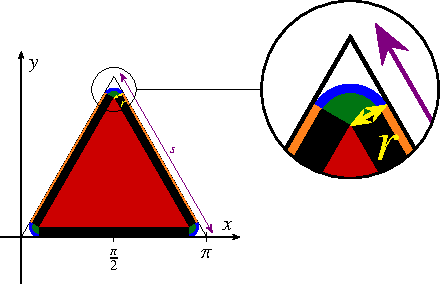
\includegraphics{papers/antennen/images/aufteilungDreieckZoom.pdf}
	\caption{Aufteilung des Dreiecks mit Zoom auf eine Ecke.}
	\label{antennen:tikzdreieckAufteilung}
\end{figure}

Durch Ableiten und Null setzten
\begin{equation}
	\frac{\partial}{\partial{r}} \bigg(\frac{l}{A^2}\bigg)=0
	\label{antennen:Ableitung}
\end{equation}
ergibt sich für eine gewünschte Seitenlänge $s$ ein Radius $r$ als Lösung. 
Die Ableitung ergibt die Gleichung 
\begin{equation}
	\frac{(- 4 \pi r + 12 \sqrt{3} r) (- 6 \sqrt{3} r + 2 \pi r + 3 s)}{\left(\pi r^{2} + 3 r (- 2 \sqrt{3} r + s) + \frac{\sqrt{3} \left(- 2 \sqrt{3} r + s\right)^{2}}{4}\right)^{3}} + \frac{- 6 \sqrt{3} + 2 \pi}{\left(\pi r^{2} + 3 r (- 2 \sqrt{3} r + s) + \frac{\sqrt{3} \left(- 2 \sqrt{3} r + s\right)^{2}}{4}\right)^{2}}=0.
	\label{antennen:Ableitunggelöst}
\end{equation}
Das Gleichungssystem hat hohen Grad. Die Lösung erfolgt numerisch, 
wobei es eine Herausforderung darstellt, mögliche und unmögliche Ergebnisse voneinander zu unterscheiden.

Als konkretes Beispiel wird der Parameter $s$, also die Seitenlänge des Dreiecks mit dem Wert $\pi$ definiert. 
Nach dem Lösen der Gleichung \eqref{antennen:Ableitunggelöst} mit dem Python-Skript \cite{antennen:codeAbleitung} erhält
man den Wert $r\approx0.2465$. Das Verhältnis zwischen Seitenlänge und Radius ist somit $\frac{\pi}{0.2465} \approx 12.744$.
Dieses Verhältnis kann nun für beliebige Seitenlängen verwendet werden und stellt somit eine wertvolle Hilfe für 
diejenigen dar, die eine optimale dreieckige Loop-Antenne entwerfen möchten.

\subsection{Fazit\label{antennen:fazit}}
In diesem Kapitel wurde eine dreieckige Antennenform ermittelt, welche die optimale Effizienz aufweist. Mittels dem Variationsprinzip von Ritz wurde dargelegt, dass eine Antenne in Form eines gleichseitigen Dreiecks für eine Effizienzsteigerung abgerundete Ecken benötigt. Das Verhältnis zwischen Seitenlänge und Radius $\frac{\pi}{0.2465} \approx 12.744$ ist optimal.



\printbibliography[heading=subbibliography]
\end{refsection}
